% This file now focuses on the book-specific content and uses shared
% preprocess/postprocess files from the project root.

% Book-specific metadata (overrides defaults in preprocess.tex)
\def\BookTitle{My Math Notes}
\def\BookAuthor{Ming Lu} % or another author if you like

% Index page offset: controls how much we shift page numbers in \hyperpage.
% This is used in postprocess.tex; adjust here per-book as needed.
\def\IndexPageOffset{0}


\input{../preprocess}

%----------------------------------------------------------------------------------------
%	Main Content
%----------------------------------------------------------------------------------------
\chapter*{Preface}
\thispagestyle{plain} % Ensure plain pagestyle is applied (with page numbers in footer)
\addcontentsline{toc}{chapter}{Preface}
Modern life feels unhinged. Modern technologies drive me crazy; every day I am flooded with loud, trivial, and overwhelming news. The United States edges toward war with Iran. Energy is becoming more expensive while Germany, having shut down its nuclear power stations years ago, now finds it difficult to restart them. France struggles to form a stable government, even as its deficits need to be paid.

I have no desire to escape to an Asian monastery in search of peace. A life that simple might be quiet, but for me it would be a waste of time. Instead, I want to focus on something that does not change, something that, ideally, only I can do. The human brain grasps stories easily and tries to make sense of them, even when there is no real sense to be found. At the same time, the human brain is notoriously bad at statistics and probabilities.

Casanova’s life is a useful example. It is tempting to look only at his adventures, but what interests me is that he helped the French government sell state lotteries to raise money, and he made a fortune doing it. Later, he lost that fortune at the gambling tables. Both his rise and his ruin were tied to probability.

Ed Thorp managed to beat the blackjack dealers using statistics, at a time when his peers insisted it was impossible. Even scientists—people who should have known better—were making confident, unscientific claims.

Now I live in Greece, where people play the lottery constantly. Everyone repeats that it is impossible to beat, and their certainty reminds me of Thorp’s colleagues. Yet at the heart of every lottery sits a random number generator, and designing a truly good one is much harder than most people think.

Knowledge of statistics and probability is always useful. I hope I can use it not only to understand these games more clearly, but also, perhaps, to earn some money.

\vspace{2em}
\begin{flushright}
Ming Lu\\
\emph{Aegina, Greece}\\
\emph{December 19, 2025}
\end{flushright}


\chapter{Why I Should Learn Math}
Millions of children hate math, and often for good reasons: the content feels
dry, the teaching feels lifeless, and many successful people seem to live well
without mathematics.

So let us ask the question honestly: why should I learn math?  Why sit in class
learning \(1+1\) when watching a movie feels far more enjoyable?

\section{Bad Answers}

I asked AI, and it gave me the usual textbook answers.  Below I separate each
\textbf{Answer} from \textbf{My critique}.

\subsection*{Answer 1}
\begin{quote}
``Learning math is essential because it enhances problem-solving skills,
supports daily life decisions, strengthens cognitive abilities, and fosters
creativity.  Practical applications in daily life include cooking, budgeting,
discounts, time management, travel planning, and home projects.''
\end{quote}

\subsection*{My Critique 1}
Come on.  A great chef does not stand in the kitchen doing explicit
calculations all day.  He or she knows what to do and when to do it, often by
experience and judgment.

\subsection*{Answer 2}
\begin{quote}
``Studying math strengthens your brain by improving memory, logical reasoning,
and analytical thinking.  Math problem-solving teaches you to identify relevant
information and apply systematic strategies that transfer to life and work.''
\end{quote}

\subsection*{My Critique 2}
I do not buy this when it is presented as a slogan.  Too often it sounds like
an unmotivated, unhappy teacher trying to convince students of something he
does not fully believe himself.

\subsection*{Answer 3}
\begin{quote}
``Math is foundational for many careers, especially STEM, finance, and
technology.  It also builds precision, objectivity, critical thinking, and
persistence, which help in almost any profession.''
\end{quote}

\subsection*{My Critique 3}
There are many rich people -- soccer players, actors, singers -- who are not
known for being strong at math.  So ``learn math to become successful'' sounds
unconvincing if success is measured only by money or fame.

\section{My Friend's Answer}
A friend of mine runs a startup and has four children.  One day, his
first-grade daughter Luisa asked why she needed to learn math.

At first he gave the usual abstract answer: ``As a business owner, I need to
understand income and expenses.''  Then he made it concrete: ``How about we
bake some cakes, sell them, and calculate profit and loss together?''

They bought ingredients, baked the cakes, and brought them first to the school
bus and then to school.

It became a small sensation.  Even the school drivers loved the cakes, and they
became a topic of conversation for the whole day.

I do not know whether Luisa fully understood the profit-and-loss calculation.
But she clearly had fun, and the math finally had a real context.

\section{My Answer}

\subsection*{Case 1: Ed Thorp and Blackjack}
Ed Thorp did not come from wealth.  He used mathematics to attack a concrete
question: what are the true odds in blackjack if cards are not replaced
immediately?  By computing conditional probabilities and expected value under
different deck compositions, he showed that the game can shift from house edge
to player edge in specific states.

To scale the strategy
into real money, he needed outside capital; one famous story is that he even
used newspaper ads to find backers, and one sponsor reportedly had underworld
connections. That was not just theory.  Casinos reacted.  He and his teammates had to use
disguises and operational discipline to avoid detection.  

The point is not glamour.  The point is precision: math turned ``I feel lucky''
into a quantified edge.

\subsection*{Case 2: LTCM and Model Risk}
Long-Term Capital Management (LTCM) had elite people and sophisticated models.
They were not ignorant of mathematics; they relied on it heavily.  But they
treated their model assumptions as if they were stable laws of nature.

Their positions were built on spreads that looked historically safe and mean
reverting.  When market conditions changed sharply, correlations moved, liquidity
dried up, and losses exploded faster than their risk framework expected.  The
fund nearly collapsed the financial system and required a coordinated rescue.

This is the second lesson: bad math, or good math used with false assumptions,
can destroy you.  Learning math is not only about finding opportunities; it is
also about understanding model limits, tail risk, and what can go wrong when
the world refuses to follow your equations.

\subsection*{Case 3: Voltaire and the French Lottery}
Historically, Voltaire (Fran\c{c}ois-Marie Arouet, 1694--1778) was one of the
central figures of the French Enlightenment: a prolific writer, satirist, and
public intellectual known for works such as \emph{Candide}, and for his
criticism of intolerance and abuse of power.

Voltaire is remembered as a writer and philosopher, but he also became wealthy
through a mathematically informed lottery strategy in France.  He and his
partners noticed a pricing flaw in the state lottery: under certain structures
of ticket pricing and payouts, buying enough tickets could create a positive
expected value.

This was not blind gambling.  It was arithmetic: identify a mispriced system,
size the participation, and repeat while the edge exists.  Voltaire's fortune
was built less by luck than by exploiting a structural inconsistency that most
people did not quantify.

\subsection*{Case 4: Casanova and the Same Lottery}
Giacomo Casanova (1725--1798), according to memoirs and historical accounts,
was not only a famous libertine adventurer but also a diplomat, writer,
occasional spy, and social operator who moved through courts and salons across
Europe.  He became widely known for his autobiography \emph{Histoire de ma vie}
(\emph{The Story of My Life}).

Casanova, in contrast, made money by helping promote and sell the same French
lottery.  He understood the social psychology around it and turned that into
wealth.

But later he was ruined by gambling losses.  The same man who benefited from a
system with engineered odds lost control when facing games where the odds were
against him.  The practical lesson is sharp: understanding one profitable setup
does not protect you if you misread probability in another.

\section{Conclusion}
You do not need to learn math to live a great life.  Running a fund like LTCM
and blowing up, or escaping prison in Venice and later going broke at gambling
tables, is also a kind of great life story.

So the choice is yours.  Do you want to be simple and rich like Voltaire and
Thorp, or spectacular and broke like LTCM or Casanova?
\chapter{Fitch Cheney's Card Trick}

\section{The Story}
You are the magician. A volunteer shuffles a normal deck. Your partner stands
next to the table. You leave the room for a moment.

When you come back, you glance at four face-up cards and immediately name the
fifth card that is hidden face down. The audience freezes for a second, then
starts laughing, shouting, and accusing you of witchcraft.

But there is no mirror, no marked deck, and no secret talking. The miracle is
pure structure: a tiny encoding system hidden in card order.

For clarity, we will still call your partner \textbf{Alice} and the magician
\textbf{Bob}.

\section{What the Audience Sees}
\begin{enumerate}
  \item A volunteer shuffles the deck and randomly chooses \(5\) cards.
  \item Bob leaves the room, so he cannot see anything.
  \item Alice looks at the \(5\) chosen cards, hides one card face down, and
  lays the other \(4\) cards face up in a specific order.
  \item Bob comes back, looks only at those \(4\) visible cards, and names the
  hidden fifth card exactly.
\end{enumerate}

To the audience, it looks impossible. There is no marked deck, no mirrors, and
no code words. The secret is pure combinatorics.

\section{Reveal: How the Trick Works}
\subsection*{Key idea}
With \(4\) visible cards, Alice can arrange them in \(4! = 24\) different ways.
So she can encode one of \(24\) possibilities by order alone.

\subsection*{Step 1: Find two cards of the same suit}
Among \(5\) cards and only \(4\) suits, at least two cards share a suit
(pigeonhole principle). Call those two same-suit cards \(X\) and \(Y\).

One of them will be shown first (the \emph{key card}), and the other one will
be hidden (the \emph{target card}).

\subsection*{Step 2: Use circular rank distance}
Within one suit, order ranks in a cycle:
\[
2,3,\dots,10,J,Q,K,A.
\]
From the key card's rank to the target card's rank, count forward distance
\(1\) to \(12\). For any two distinct ranks, one direction is at most \(6\).

Alice chooses which card is key and which is target so the forward distance is
in \(\{1,2,3,4,5,6\}\). She places the key card first.

\subsection*{Step 3: Encode distances \(1\) to \(6\) with \(3!\) orders}
After fixing the first visible card, three cards remain. Their order can be one
of \(3!=6\) permutations, perfect for encoding distances \(1\) through \(6\).

Use this fixed comparison rule:
\begin{itemize}
  \item Compare rank first: \(2<3<\cdots<K<A\).
  \item If ranks are equal, compare suit:
  \(\clubsuit<\diamondsuit<\heartsuit<\spadesuit\).
\end{itemize}
Sort the three non-key cards from small to large by this rule, and call them
\(a<b<c\).

Then agree on this encoding table:
\begin{center}
\begin{tabular}{c l}
\hline
\textbf{Distance} & \textbf{Order of last three cards} \\
\hline
1 & \(a,b,c\) \\
2 & \(a,c,b\) \\
3 & \(b,a,c\) \\
4 & \(b,c,a\) \\
5 & \(c,a,b\) \\
6 & \(c,b,a\) \\
\hline
\end{tabular}
\end{center}

Bob sees:
\begin{itemize}
  \item the first card \(\Rightarrow\) suit of the hidden card,
  \item the order of the last three \(\Rightarrow\) distance \(1\) to \(6\).
\end{itemize}
So he reconstructs the exact hidden card.

\section{Mini Example}
Suppose the five selected cards are
\[
9\heartsuit,\ K\heartsuit,\ 3\spadesuit,\ J\diamondsuit,\ 5\clubsuit.
\]
Alice decides:
\begin{itemize}
  \item key card \(=9\heartsuit\) (shown first),
  \item hidden card \(=K\heartsuit\),
  \item remaining three cards: \(3\spadesuit,\ J\diamondsuit,\ 5\clubsuit\).
\end{itemize}

From \(9\) to \(K\), the forward distance is \(4\)
\((9\to10\to J\to Q\to K)\), so Alice must encode \(4\).

Using the fixed rule above:
\[
3\spadesuit < 5\clubsuit < J\diamondsuit,
\]
so
\[
a=3\spadesuit,\quad b=5\clubsuit,\quad c=J\diamondsuit.
\]
Distance \(4\) corresponds to order \(b,c,a\), so the four visible cards are
\[
9\heartsuit,\ 5\clubsuit,\ J\diamondsuit,\ 3\spadesuit.
\]
This means Bob sees the cards in this exact left-to-right order:
\[
\boxed{9\heartsuit}\ ,\ \boxed{5\clubsuit}\ ,\ \boxed{J\diamondsuit}\ ,\ \boxed{3\spadesuit}.
\]
From the first card, Bob gets the hidden suit \(\heartsuit\). From
\(5\clubsuit,J\diamondsuit,3\spadesuit\), he reads order \(b,c,a\), so distance
\(=4\). Therefore Bob announces \(K\heartsuit\).

\subsection*{Another Example (Hide the Lower Card)}
Now consider the same-suit pair \(2\clubsuit\) and \(K\clubsuit\). If Alice used
\(2\clubsuit\) as key and tried to hide \(K\clubsuit\), the forward distance
would be \(11\), which is too large for our \(1\) to \(6\) code.

Take a full hand:
\[
2\clubsuit,\ K\clubsuit,\ 7\heartsuit,\ 4\spadesuit,\ Q\diamondsuit.
\]
So Alice reverses the direction: she \emph{shows} \(K\clubsuit\) first and
\emph{hides} \(2\clubsuit\). Then the forward distance is
\[
K\to A\to 2,
\]
which is distance \(2\).

The remaining three are \(7\heartsuit,\ 4\spadesuit,\ Q\diamondsuit\). Under
the same fixed rule:
\[
4\spadesuit < 7\heartsuit < Q\diamondsuit,
\]
so
\[
a=4\spadesuit,\quad b=7\heartsuit,\quad c=Q\diamondsuit.
\]
Distance \(2\) corresponds to order \(a,c,b\), so Alice lays out:
\[
K\clubsuit,\ 4\spadesuit,\ Q\diamondsuit,\ 7\heartsuit
\]
with \(2\clubsuit\) hidden.
So Bob sees, in exact order:
\[
\boxed{K\clubsuit}\ ,\ \boxed{4\spadesuit}\ ,\ \boxed{Q\diamondsuit}\ ,\ \boxed{7\heartsuit}.
\]
From the first card he gets suit \(\clubsuit\). From
\(4\spadesuit,Q\diamondsuit,7\heartsuit\), he reads \(a,c,b\), so distance
\(=2\). Starting at \(K\clubsuit\), two steps forward in the cycle gives
\(2\clubsuit\), which is the hidden card.

This example is important: sometimes Alice must hide the numerically lower card
to keep the distance in \(\{1,2,3,4,5,6\}\).

\section{Perform It at Home}
You can learn this in one evening. Practice with a friend:
\begin{enumerate}
  \item Memorize the distance table \(1\) to \(6\).
  \item Agree on one strict ordering rule for comparing cards.
  \item Drill 20 random hands of 5 cards and time yourselves.
  \item Start slow and accurate, then speed up.
\end{enumerate}

After a little practice, you can perform this at dinner or a party. It is a
great example of how mathematics can feel like mind reading.

\section*{Reference}
The explanation follows the MIT note by Kleber \cite{kleber:fitch-cheney}.

\chapter{Rock-Paper-Scissors}

\section{A Small Game, A Serious Battle}
Nikos and Eleni are two children in the school yard. They play
rock-paper-scissors every day.

At first, they laugh and play for fun. But soon the game becomes a real
competition. Nikos wants to prove he can read Eleni's mind. Eleni wants to show
that she can never be predicted. Both of them want to win, not just once, but
again and again.

That is what makes this tiny game interesting: the rules are simple, but the
battle is psychological. If your opponent can guess your next move, you lose.
If you can stay unpredictable, you survive.

\section{Rules of the Game}
Each player chooses one of three symbols at the same time:
\begin{itemize}
  \item Rock
  \item Paper
  \item Scissors
\end{itemize}

The winner is decided by these three relations:
\begin{itemize}
  \item Rock beats scissors.
  \item Scissors beats paper.
  \item Paper beats rock.
\end{itemize}

If both players choose the same symbol, the round is a draw.

So there are only three possible outcomes in each round:
\begin{itemize}
  \item Player A wins
  \item Player B wins
  \item Draw
\end{itemize}

\section{Nikos always plays rock}
Nikos decides to use a fixed strategy: he will always choose rock.

At first, this feels powerful to him. When Eleni picks scissors, he wins. When
she picks rock, the round is a draw. Only paper can beat him.

In the first few rounds, Nikos gets some quick wins and becomes confident. But
Eleni watches carefully. After enough rounds, she recognizes the pattern:
Nikos never changes.

Once the pattern is visible, Nikos is in trouble. Eleni can simply choose paper
more often and win again and again. The strategy that looked strong becomes easy
to exploit because it is predictable.

\section{Second stage: a 3-round cycle}
Nikos now changes strategy. Every three rounds, he plays:
\[
\text{rock} \rightarrow \text{scissors} \rightarrow \text{paper} \rightarrow \text{rock} \rightarrow \cdots
\]

At first glance, this looks much better than repeating only rock. The moves are
mixed, and Eleni cannot exploit him instantly.

However, this strategy is still fully predictable once the cycle is discovered.
After observing a few rounds, Eleni can infer Nikos's next move:
\begin{itemize}
  \item if this round is rock, next is scissors;
  \item if this round is scissors, next is paper;
  \item if this round is paper, next is rock.
\end{itemize}

So Eleni can prepare the winning counter one step ahead. This second stage is
more sophisticated than stage one, but it is still a fixed pattern.

\section{Third stage: shuffled triples}
Nikos improves again. He now uses this rule:
\begin{quote}
In every block of three rounds, I will play exactly one rock, one scissors, and
one paper, but the order can change from block to block.
\end{quote}

This sounds much harder to read. There is no single repeated sequence like
``rock, scissors, paper'' anymore.

Still, Eleni can exploit the structure \emph{inside each 3-round block}:
\begin{itemize}
  \item She watches rounds 1 and 2 of the block.
  \item Since each symbol must appear exactly once in the block, she knows the
  only symbol Nikos has not used yet.
  \item In round 3, she plays the symbol that beats that missing one.
\end{itemize}

Example:
\begin{itemize}
  \item Round 1: Nikos plays rock.
  \item Round 2: Nikos plays paper.
  \item Then round 3 must be scissors.
  \item So Eleni plays rock in round 3 and wins.
\end{itemize}

So Nikos has removed one pattern (fixed order), but kept another constraint
(exactly one of each symbol per three rounds). Eleni uses that constraint as
information and turns it into an advantage.

\section{Conclusion: Unpredictability is the key}
The story teaches one central lesson: in repeated rock-paper-scissors, being
truly unpredictable is the key.

A practical way for Nikos is to randomize in advance. For example, he can throw
dice privately and write his future moves on a paper:
\begin{itemize}
  \item \(1,2 \rightarrow\) rock
  \item \(3,4 \rightarrow\) scissors
  \item \(5,6 \rightarrow\) paper
\end{itemize}
As long as Eleni has never seen that paper, she cannot exploit a pattern in
real time.

When both players use this kind of independent randomization, they reach a
stable strategic point called a \textbf{Nash equilibrium}: no player can improve
their expected result by changing strategy alone.

In this equilibrium, each move is played with probability \(1/3\), so for each
player the long-run outcomes are:
\begin{itemize}
  \item win with probability \(1/3\),
  \item lose with probability \(1/3\),
  \item draw with probability \(1/3\).
\end{itemize}
At that point, the game is fair and neither side can gain a systematic edge.

\section{A Real Story: Choosing an Auction House}
Rock-paper-scissors is not only a children's game. It has been used in a famous
high-stakes business decision.

In 2005, Japanese executive Takashi Hashiyama wanted to sell a valuable art
collection (including works by C\'ezanne, Picasso, and Van Gogh). Two major
auction houses, Christie's and Sotheby's, both wanted the sale. Since he viewed
both proposals as strong, he asked them to settle the choice by playing
rock-paper-scissors.

Christie's reportedly asked advice from an 11-year-old girl, who suggested
scissors. Sotheby's chose paper. Scissors beat paper, so Christie's won the
right to run the auction.

This story is a perfect example of the chapter's theme: even in serious
financial settings, people sometimes rely on simple game-theoretic mechanisms
to make a fair, decisive choice \cite{wiki:rock-paper-scissors}.

\chapter{Inclusion--Exclusion Principle}
\index{Inclusion--Exclusion Principle}

\section{Why We Need It}
When we count things in two groups, it is easy to accidentally count some
objects twice.

For example, suppose:
\begin{itemize}
  \item set \(A\) is students who play football;
  \item set \(B\) is students who play basketball.
\end{itemize}

If we do \(|A| + |B|\), students who play \emph{both} sports are counted twice.
So we must subtract the overlap once.

\section{Two-Set Formula}
For two finite sets \(A\) and \(B\), the inclusion--exclusion principle says
\[
  |A \cup B| = |A| + |B| - |A \cap B|.
\]

In words:
\begin{enumerate}
  \item include \(|A|\),
  \item include \(|B|\),
  \item exclude the overlap \(|A \cap B|\) once.
\end{enumerate}

\section{A Venn Diagram}
Figure~\ref{fig:venn-two-sets} shows the two-set case.  The overlapping region
\(A \cap B\) is exactly the part that would be double-counted if we used
\(|A|+|B|\) only.

\begin{figure}[htbp]
  \centering
  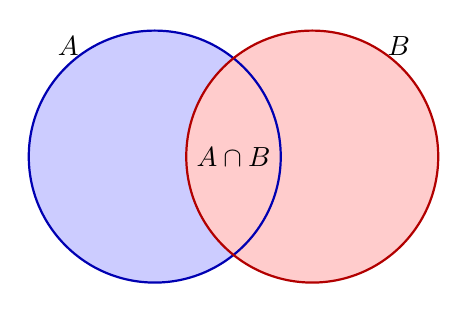
\begin{tikzpicture}[scale=1.0]
    \fill[blue!20] (-1.0,0) circle (1.6);
    \fill[red!20]  (1.0,0)  circle (1.6);
    \draw[thick, blue!70!black] (-1.0,0) circle (1.6);
    \draw[thick, red!70!black]  (1.0,0)  circle (1.6);
    \node at (-2.1,1.4) {\(A\)};
    \node at (2.1,1.4) {\(B\)};
    \node at (0,0) {\(A\cap B\)};
  \end{tikzpicture}
  \caption{Venn diagram for two sets \(A\) and \(B\).}
  \label{fig:venn-two-sets}
\end{figure}

\section{Three Sets}
For three sets \(A,B,C\), the same idea continues:
\[
  |A\cup B\cup C|
  = |A|+|B|+|C|
  - |A\cap B|-|A\cap C|-|B\cap C|
  + |A\cap B\cap C|.
\]

Why the last \(+\) term?
\begin{itemize}
  \item First we add \(|A|+|B|+|C|\): overlaps are overcounted.
  \item Then we subtract pairwise overlaps: this fixes most double counting.
  \item But the center region \(A\cap B\cap C\) was subtracted too many times,
        so we add it back once.
\end{itemize}

\section{From Three Sets to the General Pattern}
The jump from three sets to \(n\) sets is just the same correction process,
repeated one level further each time.

Think about an element \(x\) that belongs to exactly \(r\) of the sets
\(A_1,\dots,A_n\).  In the formula, this element is counted:
\begin{itemize}
  \item \(+\binom{r}{1}\) times in the ``single-set'' part,
  \item \(-\binom{r}{2}\) times in the pair-intersection part,
  \item \(+\binom{r}{3}\) times in the triple-intersection part,
  \item and so on, with alternating signs.
\end{itemize}

So the net coefficient of \(x\) becomes
\[
  \binom{r}{1} - \binom{r}{2} + \binom{r}{3} - \cdots + (-1)^{r+1}\binom{r}{r}.
\]
By the binomial identity \((1-1)^r=0\), this alternating sum equals \(1\).
That means every element in the union is counted exactly once, no matter how
many sets contain it.

This is the key reason the general formula works: each stage corrects the
over-correction made by the previous stage, and the alternating signs are
forced by this logic.

\section{General Formula}
For \(n\) sets \(A_1,\dots,A_n\):
\[
  \left|\bigcup_{i=1}^{n} A_i\right|
  =
  \sum_{i=1}^{n}|A_i|
  - \sum_{1\le i<j\le n}|A_i\cap A_j|
  + \sum_{1\le i<j<k\le n}|A_i\cap A_j\cap A_k|
  - \cdots
  + (-1)^{n+1}\left|\bigcap_{i=1}^{n}A_i\right|.
\]

The last sign is \(+\) when \(n\) is odd and \(-\) when \(n\) is even, exactly
following the alternating pattern.

Pattern to remember:
\begin{itemize}
  \item add single sets,
  \item subtract pair intersections,
  \item add triple intersections,
  \item subtract quadruple intersections,
  \item continue alternating signs.
\end{itemize}

\section{Why It Matters}
Inclusion--exclusion is a core counting tool in combinatorics and probability.
It appears in many topics, such as:
\begin{itemize}
  \item counting surjective functions,
  \item coupon collector formulas,
  \item probability of ``at least one event happens.''
\end{itemize}

Once you understand the two-set picture, the general formula is the same idea:
correct over-counting by alternating subtraction and addition.


\chapter{Euler's Totient Function and Euler's Theorem}

\section{What the Totient Function Counts}
Euler's totient function, written \(\varphi(n)\), counts how many integers from
\(1\) to \(n\) are coprime to \(n\) (that is, have greatest common divisor \(1\)
with \(n\)).\cite{wiki:euler-totient}

In symbols:
\[
  \varphi(n)=\#\{\,k \in \{1,\dots,n\} : \gcd(k,n)=1\,\}.
\]

Examples:
\begin{itemize}
  \item \(\varphi(1)=1\), because \(\gcd(1,1)=1\).
  \item \(\varphi(9)=6\), because the numbers
        \(1,2,4,5,7,8\) are coprime to \(9\), while \(3,6,9\) are not.
\end{itemize}


\section{Euler's Product Formula}
We can count the number of integers in \(\{1,\dots,n\}\) that are coprime to \(n\)
using the inclusion-exclusion principle: \index{Inclusion--Exclusion Principle}

If \(n\) has distinct prime divisors \(p_1, p_2, \dots, p_r\),
the total number \(\varphi(n)\) is n minus the multiples of \(p_i\), i=1,2,\dots,r,
plus the multiples of \(p_i\) \(p_j\), i,j=1,2,\dots,r, minus the multiples of 
\(p_i\) \(p_j\) \(p_k\), i,j,k=1,2,\dots,r, and so on.
\[
  \varphi(n)
  = n
  - \sum_{i=1}^{r}\frac{n}{p_i}
  + \sum_{1\le i<j\le r}\frac{n}{p_i p_j}
  - \sum_{1\le i<j<k\le r}\frac{n}{p_i p_j p_k}
  + \cdots
  + (-1)^r\frac{n}{p_1p_2\cdots p_r}.
\]

The result can be written as a product of the form:
\[
  \varphi(n)=n\prod_{p\mid n}\left(1-\frac{1}{p}\right).
\]

\subsection*{Example: \texorpdfstring{\(\varphi(20)\)}{phi(20)}}
Since \(20=2^2\cdot 5\),
\[
  \varphi(20)=20\left(1-\frac12\right)\left(1-\frac15\right)
  =20\cdot \frac12\cdot \frac45=8.
\]
So there are 8 integers in \(\{1,\dots,20\}\) that are coprime to \(20\).

\section{Euler's Theorem}
If \(\gcd(a,n)=1\), then
\[
  a^{\varphi(n)} \equiv 1 \pmod n.
\]

\subsection*{Elementary Proof (No Abstract Algebra)}
This proof follows the classic reduced-residue permutation argument (see
\cite{mse:euler-theorem-no-abstract-algebra}).

Let
\[
  R=\{r_1,r_2,\dots,r_{\varphi(n)}\}
\]
be all integers in \(\{1,\dots,n\}\) that are coprime to \(n\).

Multiply each element by \(a\), where \(\gcd(a,n)=1\):
\[
  ar_1,ar_2,\dots,ar_{\varphi(n)}.
\]
Reduce these modulo \(n\).  Then:
\begin{itemize}
  \item each reduced value is still coprime to \(n\), so it is again in \(R\);
  \item no two reduced values are equal modulo \(n\): if
        \(ar_i\equiv ar_j\pmod n\), then \(r_i\equiv r_j\pmod n\), hence
        \(r_i=r_j\).
\end{itemize}

So multiplication by \(a\) permutes the set \(R\).  Therefore their products are
congruent:
\[
  (ar_1)(ar_2)\cdots(ar_{\varphi(n)})
  \equiv
  r_1r_2\cdots r_{\varphi(n)}
  \pmod n.
\]
Hence
\[
  a^{\varphi(n)}(r_1r_2\cdots r_{\varphi(n)})
  \equiv
  r_1r_2\cdots r_{\varphi(n)}
  \pmod n.
\]
Because each \(r_i\) is coprime to \(n\), the product
\(r_1r_2\cdots r_{\varphi(n)}\) is also coprime to \(n\), so we can cancel it.
We get
\[
  a^{\varphi(n)} \equiv 1 \pmod n.
\]

\subsection*{Examples}
\begin{itemize}
  \item \textbf{\(a=2,\ n=5\):} \(\gcd(2,5)=1\) and \(\varphi(5)=4\), so Euler's theorem predicts
        \(2^4\equiv 1 \pmod 5\).  Indeed, \(2^4=16\), and \(16\equiv 1 \pmod 5\).

  \item \textbf{\(a=3,\ n=10\):} \(\gcd(3,10)=1\) and \(\varphi(10)=4\), so
        \(3^4\equiv 1 \pmod{10}\).  Indeed, \(3^4=81\), and
        \(81\equiv 1 \pmod{10}\).

  \item \textbf{\(a=2,\ n=9\):} \(\gcd(2,9)=1\) and \(\varphi(9)=6\), so
        \(2^6\equiv 1 \pmod 9\).  Indeed, \(2^6=64\), and \(64\equiv 1 \pmod 9\).

  \item \textbf{\(a=5,\ n=12\):} \(\gcd(5,12)=1\) and \(\varphi(12)=4\), so
        \(5^4\equiv 1 \pmod{12}\).  Indeed, \(5^2=25\equiv 1 \pmod{12}\), hence
        \(5^4=(5^2)^2\equiv 1^2\equiv 1 \pmod{12}\).
\end{itemize}

The theorem can be used to reduce large powers modulo \(n\).  For example, to
find the ones digit of \(7^{222}\), compute \(7^{222}\pmod{10}\).  Since
\(\gcd(7,10)=1\) and \(\varphi(10)=4\), Euler's theorem gives
\[
  7^4 \equiv 1 \pmod{10}.
\]
Now write \(222 = 4\cdot 55 + 2\).  Then
\[
  7^{222}
  \equiv 7^{4\cdot 55 + 2}
  \equiv (7^4)^{55}\cdot 7^2
  \equiv 1^{55}\cdot 7^2
  \equiv 49
  \equiv 9 \pmod{10}.
\]
So the ones digit of \(7^{222}\) is \(9\).



Euler's theorem is one of the reasons \(\varphi(n)\) is so important in
cryptography: RSA relies on this modular-exponentiation structure.

\chapter{RSA Cryptosystem}

\section{What is RSA?}
RSA is one of the most famous public-key cryptosystems. It lets people
communicate securely without first sharing a secret key.

The core idea is simple:
\begin{itemize}
  \item A \textbf{public key} is shared with everyone and is used to encrypt.
  \item A \textbf{private key} is kept secret and is used to decrypt.
\end{itemize}

RSA is also used for digital signatures, but in this chapter we focus on
encryption/decryption and the mathematical principle behind why it works.

\subsection*{Alice, Bob, and Eve}
Think of three people:
\begin{itemize}
  \item \textbf{Alice}: wants to receive a secret message.
  \item \textbf{Bob}: wants to send the message.
  \item \textbf{Eve}: can eavesdrop on every message sent over the network.
\end{itemize}

Alice publishes her \textbf{public key}. Bob uses that public key to encrypt.
Eve can see the public key and the ciphertext, but cannot recover the plaintext
without Alice's private key. Alice then uses her private key to decrypt.

So the story is:
\begin{enumerate}
  \item Alice generates keys and publishes \((n,e)\).
  \item Bob computes \(c\equiv m^e\pmod n\) and sends \(c\).
  \item Eve sees \(c\), but should not be able to get \(m\).
  \item Alice computes \(m\equiv c^d\pmod n\) and recovers the message.
\end{enumerate}

\section{Key Generation}
Choose two large prime numbers \(p\) and \(q\), then define
\[
  n = pq.
\]
Compute
\[
  \varphi(n) = (p-1)(q-1).
\]
Choose an integer \(e\) such that
\[
  1 < e < \varphi(n), \qquad \gcd(e,\varphi(n))=1.
\]
Then choose \(d\) such that
\[
  ed \equiv 1 \pmod{\varphi(n)}.
\]
The public key is \((n,e)\), and the private key is \((n,d)\).

\section{Encryption and Decryption}
Represent a message as an integer \(m\) with \(0 \le m < n\).

\textbf{Encryption:}
\[
  c \equiv m^e \pmod n.
\]

\textbf{Decryption:}
\[
  m \equiv c^d \pmod n.
\]

In words: raise to \(e\) to encrypt, raise to \(d\) to decrypt.

In the Alice-Bob-Eve picture:
\begin{itemize}
  \item Bob uses Alice's public key \((n,e)\) to compute \(c\).
  \item Eve can read \(c\), but she does not know Alice's \(d\).
  \item Alice uses \(d\) to recover \(m\).
\end{itemize}

\section{Small Numerical Example}
For teaching, we use small numbers (in practice, primes are much larger):
\[
  p=61,\quad q=53.
\]
Then
\[
  n = pq = 3233,\qquad \varphi(n)=(61-1)(53-1)=3120.
\]
Pick
\[
  e=17,\qquad \gcd(17,3120)=1.
\]
Find \(d\) from \(ed\equiv 1 \pmod{3120}\), which gives
\[
  d=2753
\]
because \(17\cdot 2753 = 46801 = 3120\cdot 15 + 1\).

So:
\begin{itemize}
  \item Public key: \((n,e)=(3233,17)\)
  \item Private key: \((n,d)=(3233,2753)\)
\end{itemize}

Encrypt message \(m=65\):
\[
  c \equiv 65^{17} \pmod{3233} = 2790.
\]

Decrypt:
\[
  m \equiv 2790^{2753} \pmod{3233} = 65.
\]
So the original message is recovered.

\section{Why RSA Works}
The proof of correctness is based on Fermat's little theorem:
if \(p\) is prime and \(p\nmid a\), then
\[
  a^{p-1}\equiv 1 \pmod p.
\]

We want to show
\[
  (m^e)^d \equiv m \pmod{pq}
\]
for every integer \(m\), where \(p\) and \(q\) are distinct primes, and \(e,d\)
satisfy
\[
  ed \equiv 1 \pmod{\varphi(pq)}.
\]


\begin{enumerate}
  \item gcd(m, pq) \neq 1, 

  Both p and q are primes. m must be multiple of p or q. let's assume m is multiple of p. m = pk. m is multiple
  \[
    m^{ed}
    =(pk)^{ed}
    \equiv 0 
    \equiv m \pmod p
  \]

  \[
    m^{ed}
    =m^{ed-1}m
    =m^{k(q-1)}m
    \equiv m \pmod q
  \]

  We have therefore
  \[
    m^{ed}=qx+m
  \]
  Since $m^{ed}$ is multiple of p, m is multiple of p, we have x is multiple of p.
  \[
    m^{ed}=pq(x/p)+m
    \equiv m \pmod {pq}
  \]

  \item gcd(m, pq) = 1, 
  We can use Euler's theorem to prove directly.
  \[
    m^{ed}
    =m^{ed-1}m
    =m^{k\varphi(pq)}m
    \equiv 1^k m
    \equiv m
    \pmod {pq}
  \]
\end{enumerate}

Therefore \(m^{ed}\equiv m\pmod p\) and \(m^{ed}\equiv m\pmod q\), so
\[
  (m^e)^d \equiv m \pmod{pq}.
\]
This proves correctness for every integer \(m\).

\section{Modular Exponentiation}
At this point, a practical question appears:
\[
  m \equiv 2790^{2753} \pmod{3233}.
\]
How can we compute this without multiplying \(2790\) by itself 2753 times?

The naive method is too slow for real RSA. In practice, exponents are huge
(hundreds or thousands of bits), so we must use a smarter method.

The standard trick is \textbf{binary exponentiation} (also called
square-and-multiply). It uses:
\[
  a^b=
  \begin{cases}
    (a^{b/2})^2, & b \text{ even},\\[2mm]
    a\,(a^{(b-1)/2})^2, & b \text{ odd}.
  \end{cases}
\]
So instead of reducing the exponent by \(1\) each step, we roughly halve it
each step. That is why the complexity is \(O(\log b)\), not \(O(b)\).

We also reduce modulo \(n\) at every multiplication:
\[
  (xy)\bmod n = \bigl((x\bmod n)(y\bmod n)\bigr)\bmod n.
\]
This keeps numbers small during the whole computation.

Here is a clean recursive implementation:
\begin{lstlisting}[language=Python]
def fast_expo_modulo(base: int, exp: int, modulo: int):
    if exp==1:
        return base%modulo
    if exp ==0:
        return 1
    if exp % 2 == 1:
        return (fast_expo_modulo(base, (exp-1)/2, modulo) %modulo* 
            fast_expo_modulo(base, (exp-1)/2, modulo) %modulo 
            * (base%modulo))%modulo
    else:
        return (fast_expo_modulo(base, exp/2, modulo) %modulo* 
            fast_expo_modulo(base, exp/2, modulo) %modulo) %modulo
\end{lstlisting}

\section{Computing the Private Key with Extended Euclid}
In RSA key generation, after choosing \(e\), we must compute the private key
exponent \(d\) from
\[
  ed \equiv 1 \pmod{\varphi(n)}
\]
(or modulo \(\lambda(n)\) in many implementations). So \(d\) is the
\textbf{modular multiplicative inverse} of \(e\).

The Extended Euclidean Algorithm gives exactly this inverse. Since
\(\gcd(e,\varphi(n))=1\), it finds integers \(x,y\) such that
\[
  ex+\varphi(n)y=1.
\]
Taking both sides modulo \(\varphi(n)\):
\[
  ex \equiv 1 \pmod{\varphi(n)}.
\]
Therefore \(x\) is an inverse of \(e\), so we can take
\[
  d \equiv x \pmod{\varphi(n)}.
\]
If \(x<0\), convert it to a positive representative by adding \(\varphi(n)\).
This is the standard method used in RSA implementations \cite{wiki:rsa-cryptosystem,wiki:modular-multiplicative-inverse}.

\subsection*{How the algorithm works (and why)}
The ordinary Euclidean algorithm repeatedly applies division with remainder:
\[
a=bq+r,\qquad 0\le r<b.
\]
Then \(\gcd(a,b)=\gcd(b,r)\). Repeating this step makes numbers smaller until
the remainder is \(0\), and the last nonzero remainder is the gcd.

The \emph{extended} Euclidean algorithm keeps extra bookkeeping: at each step,
it remembers how the current remainder is written as a linear combination of
the original two numbers. So every remainder has the form
\[
r_i = s_i a + t_i b.
\]
When the gcd is \(1\), this finally gives
\[
1 = sa+tb.
\]
This identity is called a B\'{e}zout identity.

Now apply it to RSA with \(a=e\) and \(b=\varphi(n)\):
\[
1 = se + t\varphi(n).
\]
Reduce modulo \(\varphi(n)\):
\[
se \equiv 1 \pmod{\varphi(n)}.
\]
So \(s\) is exactly \(e^{-1}\bmod \varphi(n)\), i.e. the private exponent
\(d\) (up to adding multiples of \(\varphi(n)\)).

\subsection*{Worked Example}
Use the chapter's RSA toy parameters:
\[
  e=17,\qquad \varphi(n)=3120.
\]
Euclidean steps:
\[
3120=183\cdot17+9,\quad
17=1\cdot9+8,\quad
9=1\cdot8+1.
\]
Back-substitute:
\[
\begin{aligned}
1&=9-1\cdot8\\
 &=9-(17-1\cdot9)=2\cdot9-17\\
 &=2(3120-183\cdot17)-17\\
 &=2\cdot3120-367\cdot17.
\end{aligned}
\]
So
\[
17(-367)+3120(2)=1.
\]
Hence
\[
17(-367)\equiv1\pmod{3120},
\]
and the private exponent is
\[
d\equiv -367\equiv 2753\pmod{3120}.
\]
This is exactly the \(d\) used earlier in the chapter.

\section{Practical Notes}
\begin{itemize}
  \item Real RSA uses very large primes (typically 2048-bit keys or larger).
  \item RSA security relies on the difficulty of factoring large integers.
\end{itemize}

\section*{Reference}
This chapter follows the standard RSA description in \cite{wiki:rsa-cryptosystem}.

\chapter{Greek PowerSpin Lottery}
\section{Rules of PowerSpin}

PowerSpin is a wheel game with 27 possible outcomes:
\begin{itemize}
\item 24 numbered positions: $1,2,\ldots,24$
\item 3 special PowerSpin symbol positions
\end{itemize}

Each round proceeds as follows:
\begin{enumerate}
\item Players place their bets predicting the outcome of the next spin.
\item The wheel is spun once.
\item The result is either one of the numbers $1$--$24$ or a PowerSpin symbol.
\item If the result matches the prediction, the player wins according to the payout table.
\end{enumerate}

Players may choose among several types of predictions:
\begin{itemize}
\item A single number.
\item A group of numbers (2, 3, 4, 6, 8, or 12 numbers).
\item A color zone (one of three zones, each containing 8 numbers).
\item A PowerSpin symbol.
\item Over/Under $12.5$ (numbers $1$--$12$ or $13$--$24$).
\end{itemize}

\section{Payouts}

If a prediction is correct, the stake is multiplied by the corresponding multiplier shown in the official PowerSpin payout table published by OPAP.

\subsection{Single Wheel Bets}

\begin{center}
\begin{tabular}{ll}
\textbf{Game Type} & \textbf{Multiplier} \\
Number & $\times 24$ \\
Double (2 numbers) & $\times 12$ \\
Triple (3 numbers) & $\times 8$ \\
Quadruple (4 numbers) & $\times 6$ \\
Sextuple (6 numbers) & $\times 4$ \\
Octuple (8 numbers) & $\times 3$ \\
Dozen (12 numbers) & $\times 2$ \\
Symbol & $\times 8$ \\
Zone & $\times 3$ \\
Over/Under $12.5$ & $\times 2$ \\
\end{tabular}
\end{center}

\subsection{Two-Wheel Combination Bets}

\begin{center}
\begin{tabular}{ll}
\textbf{Combination} & \textbf{Multiplier} \\
Number -- Number & $\times 630$ \\
Symbol -- Symbol & $\times 70$ \\
Zone -- Zone & $\times 10$ \\
Over/Under -- Over/Under & $\times 4.4$ \\
Number -- Symbol & $\times 210$ \\
Number -- Zone & $\times 80$ \\
Number -- Over/Under & $\times 54$ \\
Symbol -- Zone & $\times 27$ \\
Symbol -- Over/Under & $\times 18$ \\
Zone -- Over/Under & $\times 6.4$ \\
\end{tabular}
\end{center}

\subsection{Three-Wheel Combination Bets}

\begin{center}
\begin{tabular}{ll}
\textbf{Combination} & \textbf{Multiplier} \\
Number -- Number -- Number & $\times 17{,}000$ \\
Symbol -- Symbol -- Symbol & $\times 600$ \\
Zone -- Zone -- Zone & $\times 33$ \\
Over/Under -- Over/Under -- Over/Under & $\times 10$ \\
2 Numbers -- Symbol & $\times 5{,}500$ \\
2 Numbers -- Zone & $\times 2{,}100$ \\
2 Numbers -- Over/Under & $\times 1{,}400$ \\
2 Symbols -- Number & $\times 1{,}800$ \\
2 Symbols -- Zone & $\times 230$ \\
2 Symbols -- Over/Under & $\times 150$ \\
2 Zones -- Number & $\times 260$ \\
2 Zones -- Symbol & $\times 85$ \\
2 Zones -- Over/Under & $\times 21$ \\
2 Over/Under -- Number & $\times 120$ \\
2 Over/Under -- Symbol & $\times 40$ \\
2 Over/Under -- Zone & $\times 15$ \\
Number -- Symbol -- Zone & $\times 680$ \\
Number -- Symbol -- Over/Under & $\times 450$ \\
Number -- Zone -- Over/Under & $\times 170$ \\
Symbol -- Zone -- Over/Under & $\times 60$ \\
\end{tabular}
\end{center}
\chapter{Random Variables}

In everyday language we talk about ``random events'': a lottery draw, tomorrow's stock return, the time a bus arrives.  A \emph{random variable} is simply a way to assign a numerical value to the outcome of such an uncertain event.  For example:
\begin{itemize}
  \item let $X$ be ``the PowerSpin result'' (values $1$ to $24$ or a symbol);
  \item let $Y$ be ``the number of winning tickets'' in a given draw;
  \item let $R$ be ``tomorrow's daily return'' of a stock, measured in percent.
\end{itemize}
Each of these quantities can take different values from one trial to the next, and we do not know in advance which value we will see.  Thinking of them as random variables lets us talk precisely about their probabilities, their averages (expectations), and how much they fluctuate (variance).

This is not just a theoretical game.  In finance, misunderstanding random variables has ruined real firms.  The hedge fund LTCM (Long-Term Capital Management) in the late 1990s built strategies on the assumption that certain price spreads were extremely unlikely to move beyond a narrow range.  In effect, they treated the relevant random variables as if large deviations were almost impossible.  When rare but perfectly possible moves \emph{did} occur, the losses were far outside what their models had prepared them for, and the fund collapsed.  Understanding random variables, and especially their tails and correlations, is therefore not only mathematically interesting; it can be the difference between a robust strategy and a disaster.
\chapter{Common Distributions}

\section{Uniform Distribution}
The simplest distribution is the \emph{discrete uniform} distribution.  It
describes a random variable that takes one of a finite set of values, all with
equal probability.  Examples:
\begin{itemize}
  \item a fair six-sided dice: each of \(1,2,3,4,5,6\) has probability \(1/6\);
  \item a single PowerSpin wheel result (ignoring the symbol grouping) when each
        of the 27 positions is equally likely.
\end{itemize}

If a random variable \(X\) is uniformly distributed over
\(\{1,2,\dots,n\}\), we write
\[
  P(X = k) = \frac{1}{n}, \quad k = 1,2,\dots,n.
\]
Its mean and variance are
\[
  \mathbb{E}[X] = \frac{n+1}{2}, \qquad
  \mathrm{Var}(X) = \frac{n^2-1}{12}.
\]

Uniform distributions capture the ideal of ``no preference'' among outcomes.
They are the starting point for most lottery and dice models in this book.

\section{Geometric Distribution}
The \emph{geometric} distribution describes the number of trials needed to get
the first \emph{success} in a sequence of independent trials, each with the
same success probability \(p\).  Typical stories:
\begin{itemize}
  \item ``How many tickets do I need to buy until I win once?''
  \item ``How many times do I roll until I see my favourite number?''
\end{itemize}

Let \(X\) be the number of trials needed to get the first success.  Then
\[
  P(X = k) = (1-p)^{k-1}p, \quad k = 1,2,3,\dots
\]
That is, we fail \(k-1\) times (each with probability \(1-p\)) and then
succeed on the \(k\)-th trial.

The mean and variance of a geometric random variable are
\[
  \mathbb{E}[X] = \frac{1}{p}, \qquad
  \mathrm{Var}(X) = \frac{1-p}{p^2}.
\]

The geometric distribution appears repeatedly in this book.  In the coupon
collector's problem, each \(t_i\) (the waiting time for the next new coupon) is
geometrically distributed with a suitable success probability \(p_i\).  In
lottery testing, geometric waiting times can describe how long we expect to
wait until a rare event occurs under a fair mechanism.


\chapter{The Central Limit Theorem}

\section{Starting from Dice}
Imagine rolling a single fair six-sided dice.  Each throw is simple and familiar: you see one of the numbers \(1,2,3,4,5,6\), all equally likely.  Now consider a slightly different experiment: roll the dice several times and \emph{add up} the results.

For example:
\begin{itemize}
  \item with one throw, the result can only be \(1\) to \(6\), and all six outcomes are equally likely;
  \item with two throws, the sum can range from \(2\) to \(12\), but not all sums are equally likely --- there are many ways to make \(7\), but only one way to make \(2\);
  \item with ten throws, the sum can range from \(10\) to \(60\), and most of the probability mass is concentrated in the middle region.
\end{itemize}

If you repeat the ``sum of ten throws'' experiment many times and draw a histogram of the sums, you see a familiar shape begin to appear: a smooth, bell-like curve, highest in the middle and tapering off towards the extremes.  This is not an accident.  It is the first hint of the \emph{Central Limit Theorem}.

\section{What the Theorem Says (Informally)}
The Central Limit Theorem (CLT) can be stated informally as:
\begin{quote}
  \emph{Whenever you add up many independent random contributions of roughly similar size, the distribution of the sum tends to look more and more like a Gaussian (normal) bell curve, regardless of the original distribution of each contribution.}
\end{quote}

In the dice example, each throw is one ``contribution''.  When you add many throws, the sum behaves more and more like a Gaussian random variable --- its histogram becomes smoother and more symmetric, and the probability of being far away from the centre drops off in a way that resembles the Gaussian tail.

This phenomenon is not limited to dice.  It appears whenever a quantity is the sum of many small influences: measurement errors, daily fluctuations in demand, tiny physical forces acting together, and so on.  The CLT explains why the Gaussian distribution shows up so often in nature and in data.

\section{When the CLT Applies (and When to Be Careful)}
The CLT does not require perfection, but it does have some conditions.  In practice, it works well when:
\begin{itemize}
  \item the contributions you add are \textbf{independent} (one draw does not heavily influence the next);
  \item none of the contributions is \textbf{overwhelmingly larger} than the others (no single term dominates the sum);
  \item the underlying distribution is not too wild in its tails (extremely heavy-tailed distributions need more care).
\end{itemize}

For many everyday distributions, such as the uniform distribution on an interval, the CLT starts to give a good approximation surprisingly quickly.  A useful rule of thumb for a \textbf{uniform} distribution is:
\begin{quote}
  \emph{If you add together around 20--30 independent uniform draws (for example, 20--30 dice or lottery-like draws of equal range), the distribution of the sum is already quite close to a Gaussian.}
\end{quote}

With even more terms, the approximation improves further.  The exact number is not magical and depends on how accurate you need the approximation to be, but this gives a practical sense of scale: tens of independent contributions are often enough for the CLT to be useful in modelling sums by a Gaussian distribution.

\section{Mean and Spread in Layman Terms}
To describe the bell curve that appears, we need two basic ideas.

\subsection{The Mean (Expectation)}
The \emph{mean}, or \emph{expectation}, of a random quantity is its long-run average value.  For the dice, each face from \(1\) to \(6\) has probability \(1/6\), so the expected value of one throw is
\[
  \mathbb{E}[\text{one throw}] = \frac{1\cdot 1 + 2\cdot 1 + 3\cdot 1 + 4\cdot 1 + 5\cdot 1 + 6\cdot 1}{6}
  = \frac{1+2+3+4+5+6}{6} = 3.5.
\]
If you keep throwing the dice and averaging the results, your running average will wander around but gradually settle near \(3.5\).

In general, if a random variable \(X\) can take values \(x_1, x_2, \dots, x_k\) with probabilities \(p_1, p_2, \dots, p_k\), its expectation is
\[
  \mathbb{E}[X] = \sum_{i=1}^{k} x_i\,p_i.
\]

For the sum of ten independent throws, the mean is simply ten times larger:
\[
  \mathbb{E}[\text{sum of ten throws}] = 10 \times \mathbb{E}[\text{one throw}] = 10 \times 3.5 = 35.
\]
This is why the histogram of sums is centred near \(35\).

\subsection{How Much the Values Vary (Variance)}
The second ingredient is how much the outcomes \emph{spread out} around the mean.  In everyday language we might say:
\begin{itemize}
  \item some quantities are ``tightly concentrated'' around their average;
  \item others are ``very noisy'' or ``highly variable''.
\end{itemize}

Mathematically this spread is measured by the \emph{variance} or its square root, the \emph{standard deviation}.  For a random variable \(X\) with mean \(\mathbb{E}[X]\), the variance is defined as
\[
  \mathrm{Var}(X) = \mathbb{E}\bigl[(X - \mathbb{E}[X])^2\bigr],
\]
the expected value of the squared distance from the mean.  You can think of it as the average squared ``error'' between \(X\) and its own average.

For our purposes it is enough to remember that:
\begin{itemize}
  \item a larger variance means the values are more spread out;
  \item a smaller variance means they are more tightly clustered around the mean.
\end{itemize}

When we add many independent contributions, the mean of the sum grows in proportion to the number of terms, and the spread also grows, but in a more controlled way.  After the right rescaling, the CLT tells us that the shape we see tends towards the Gaussian bell curve.

\section{The Parameters of a Gaussian Distribution}
A Gaussian (normal) distribution is fully described by just two numbers:
\begin{itemize}
  \item its \textbf{mean} \(\mu\) (where the peak of the bell curve sits);
  \item its \textbf{variance} \(\sigma^2\) (how wide the bell is).\index{Gaussian Distribution}\index{Normal Distribution}
\end{itemize}

We write this as
\[
  X \sim \mathcal{N}(\mu, \sigma^2),
\]
which should be read as: ``the random variable \(X\) follows a Gaussian distribution with mean \(\mu\) and variance \(\sigma^2\).''  Changing \(\mu\) shifts the whole curve left or right.  Changing \(\sigma^2\) stretches it out or squeezes it in: a larger variance means a flatter, wider bell; a smaller variance means a taller, narrower bell.

In the dice example:
\begin{itemize}
  \item for one throw, the mean is \(3.5\) and the variance has some fixed value;
  \item for the sum of many throws, the mean is larger and the variance is larger, but the overall \emph{shape} of the histogram becomes more and more like a Gaussian.
\end{itemize}

The Central Limit Theorem links these ideas together: it explains why sums of many small random effects are well modelled by a Gaussian distribution with an appropriate mean and variance, and therefore why the Gaussian curve lies at the heart of statistical testing, including the chi-squared methods used elsewhere in this book.


% -------------------------------------------------------------
\chapter{The General Structure}
% -------------------------------------------------------------
 
% -------------------------------------------------------------
\section{Two Levels of Testing}
% -------------------------------------------------------------
 
When Knuth describes empirical randomness testing\cite{knuth:1997-taocp-2}, two distinct levels are
at work, and it is important not to conflate them.
 
At the \textbf{upper level} sit the \emph{empirical tests} themselves ---
the frequency test, the serial test, the gap test, the poker test, the runs
test, and so on.  Each of these tests focuses on a specific property of the
draw sequence: how often each outcome appears, how pairs of consecutive
draws relate, how long the gaps between specific outcomes are, and so forth.
Applying one of these tests means extracting a particular numerical summary
from the sequence that reflects that property.
 
At the \textbf{lower level} sit two general-purpose statistical procedures:
the \emph{chi-squared test} and the \emph{Kolmogorov--Smirnov test}.  These
are not empirical tests in their own right.  They are the machinery that
every empirical test relies on to reach a conclusion.  Once an empirical
test has reduced the data to a test statistic, it is the chi-squared or KS
procedure that converts that statistic into a $p$-value and a verdict.
 
\begin{keyidea}[The Relationship Between the Two Levels]
Every empirical randomness test described by Knuth ultimately delegates its
final decision to one of two tools: the chi-squared test or the
Kolmogorov--Smirnov test.  These two procedures are not members of the
battery of empirical tests --- they are the statistical engine that all
members of the battery run on.
\end{keyidea}
 
% -------------------------------------------------------------
\section{The General Structure of a Statistical Test}
% -------------------------------------------------------------
 
Before examining the two procedures in detail, it is worth stating the
logical structure they share.
 
Each empirical test produces a \textbf{test statistic}: a single number
computed from the observed data.  This statistic is designed so that, when
the draw sequence truly is random, the statistic follows a \emph{known
reference distribution}.  The chi-squared and KS procedures each provide
one such reference distribution.
 
The conclusion of a test is then expressed as a \textbf{$p$-value}: the
probability that a genuinely random process would produce a test statistic
at least as extreme as the one observed.  A very small $p$-value means the
data is highly inconsistent with randomness; a $p$-value near one means the
data fits the expected pattern suspiciously well.  Both extremes are cause
for investigation.
 
We choose a \textbf{significance level} $\alpha$ in advance.  If the
$p$-value falls below $\alpha$, we reject the null hypothesis that the
sequence is random.  Common choices are $\alpha = 0.05$ and $\alpha = 0.01$.
 
% -------------------------------------------------------------
\section{What Makes These Two Procedures Universal}
% -------------------------------------------------------------
 
One might ask: why do all empirical tests converge on the same two
procedures?  The answer lies in a property that both the chi-squared and KS
tests possess, which makes them applicable across a wide variety of
situations without modification.
 
\begin{keyidea}[Distribution-Free Property]
The reference distributions of the chi-squared and Kolmogorov--Smirnov test
statistics under $H_0$ do not depend on the specific probability
distribution that the data is supposed to follow.  The same reference
distribution, and the same tables of critical values, apply regardless of
whether the underlying theoretical distribution is uniform, geometric,
exponential, or any other shape.
\end{keyidea}
 
This is what allows the same two procedures to serve as the foundation for
every empirical test.  Each empirical test examines a different property and
therefore works with a different theoretical distribution --- the frequency
test works with a uniform distribution over ball numbers, the gap test works
with a geometric distribution of waiting times, the runs test works with a
combinatorial distribution of run lengths, and so on.  Despite this variety,
every one of these tests can hand its test statistic to either the
chi-squared or the KS procedure and receive a valid $p$-value in return,
because those procedures are indifferent to the shape of the underlying
distribution.
 
\begin{important}
This distribution-free property is not trivial.  Most statistical tests are
derived specifically for one type of distribution and cannot be reused
elsewhere without re-derivation.  The chi-squared and KS tests are
exceptions: their validity is guaranteed by general mathematical theorems
that hold for any distribution, making them ideal as universal foundations.
\end{important}
 
% -------------------------------------------------------------
\section{The Chi-Squared Test}\label{sec:chi-squared-test}
% -------------------------------------------------------------
\index{Chi-squared Test}

\subsection{When It Is Used}
 
The chi-squared procedure is used when the test statistic from an empirical
test takes the form of \textbf{counts in discrete categories}.  The
empirical test observes how many times each of several possible outcomes
occurred and compares those counts to how many times each outcome was
expected to occur.
 
\subsection{The Test Statistic}
 
Let there be $k$ categories.  For category $i$, let $O_i$ denote the
observed count and $E_i$ the expected count under $H_0$.  The chi-squared
statistic is:
\[
  \chi^2 = \sum_{i=1}^{k} \frac{(O_i - E_i)^2}{E_i}
\]
 
The normalisation by $E_i$ is essential: it places discrepancies from
high-probability categories and low-probability categories on the same
scale, so that each contributes comparably to the total.
 
\subsection{The Reference Distribution and Its Independence from $E_i$}
 
When $H_0$ is true, the statistic $\chi^2$ follows approximately the
\emph{chi-squared distribution with $\nu = k - 1$ degrees of freedom}.
The critical observation is that this reference distribution depends only
on the number of categories $k$, and not at all on the individual expected
values $E_1, E_2, \ldots, E_k$.
 
This means that an empirical test with ten categories always consults the
chi-squared distribution with nine degrees of freedom, regardless of whether
those ten categories each have equal probability or wildly unequal
probabilities.  The same table entry provides the $p$-value in every case.
 
\begin{keyidea}
The chi-squared statistic translates category counts --- measured against
any theoretical distribution with any shape --- into a single universal
scale.  The reference distribution depends only on how many categories there
are, not on what those categories represent or how probable they are.
\end{keyidea}
 
\subsection{What the Chi-Squared Distribution Looks Like}

For each fixed number of degrees of freedom $\nu$, there is a corresponding
\emph{chi-squared distribution}.  You can think of it as a bell-shaped
curve that has been pushed over so that it starts at $0$ and has a long
tail out to the right:\index{Chi-squared Distribution}
\begin{itemize}
  \item $\chi^2$ can never be negative, because it is a sum of squared
        discrepancies.
  \item Values near $0$ correspond to counts that match the expectations
        almost perfectly.
  \item Larger values of $\chi^2$ correspond to counts that are
        increasingly uneven.
\end{itemize}

There is also a more structural way to view this distribution.  Take a
random variable $Z$ that follows a \emph{Gaussian} (or \emph{normal})
distribution with mean $0$ and variance $1$, usually written
$Z \sim \mathcal{N}(0,1)$.  This is the familiar bell-shaped curve: it is
symmetrical around $0$, values close to $0$ are common, and very large
positive or negative values are increasingly rare.  If you square such a
variable, $Z^2$, the result follows a chi-squared distribution with
one degree of freedom.  If you take several independent such variables
$Z_1, Z_2, \dots, Z_\nu$ and add their squares,
\[
  \chi^2 = Z_1^2 + Z_2^2 + \cdots + Z_\nu^2,
\]
then $\chi^2$ has a chi-squared distribution with $\nu$ degrees of
freedom.  In this sense, chi-squared distributions describe sums of
squared Gaussian variables.

For small $\nu$ the curve is strongly skewed; for large $\nu$ it becomes
more and more symmetric and bell-like.  The important point is that, once
$\nu$ is known, the entire shape of this curve is fixed, and so is the
probability that $\chi^2$ will fall in any given range.

\subsection{How the $p$-Value Is Obtained in Practice}

Once you have computed $\chi^2$ and the degrees of freedom $\nu$, the
$p$-value is simply the probability, under the chi-squared distribution
with $\nu$ degrees of freedom, of seeing a value at least as large as the
one you observed.  There are two practical ways to obtain it:
\begin{itemize}
  \item \textbf{Using tables.}  Traditional statistics books print
        \emph{chi-squared tables} with rows for degrees of freedom and
        columns for selected upper-tail probabilities (for example
        $0.10$, $0.05$, $0.01$, $0.001$).  Given $\nu$ and your $\chi^2$
        value, you look along the row for $\nu$ to see between which two
        columns your statistic falls.  This tells you that the $p$-value
        lies between the corresponding probabilities.
  \item \textbf{Using a computer program.}  Any scientific computing
        environment (R, Python, Julia, a spreadsheet, or a statistics
        package) can evaluate the chi-squared CDF directly.  You give it
        $\chi^2$ and $\nu$, and it returns the exact upper-tail
        probability.  This is the most convenient option in modern work,
        and is what we will assume when we quote numerical $p$-values in
        later chapters.
\end{itemize}

Either way, the logic is the same: we place the observed $\chi^2$ on the
chi-squared distribution with the correct degrees of freedom and read off
how much probability lies to the right of it.  That right-hand probability
is the $p$-value.
 
\subsection{What It Is Sensitive To}
 
The chi-squared test detects discrepancies that are \emph{distributed across
many categories}.  It is powerful when multiple categories deviate
moderately from their expected counts simultaneously.  Because the test
sums contributions from all categories equally, it does not weight any
particular category more heavily than another, and it discards any ordering
among the categories.  As a result, it cannot detect trends where deviations
are systematically arranged --- for example, consistently too high in one
part of the range and too low in another.
 
\subsection{A Requirement on Expected Counts}
 
The chi-squared distribution is an approximation, and it requires each
expected count $E_i$ to be sufficiently large to be reliable.  When an
empirical test produces categories with very small expected counts, those
categories must be merged with neighbouring ones until the requirement is
met.  This changes $k$ and therefore the degrees of freedom.
 
\subsection{How to Interpret the $p$-Value (Rule of Thumb)}
\index{$p$-value}

Knuth gives a practical interpretation scheme for the $p$-values produced by
randomness tests.\cite{knuth:1997-taocp-2}  The idea is not to treat a single
test run as a final verdict, but to classify outcomes by how extreme they are.

\begin{itemize}
  \item If $p < 1\%$ or $p > 99\%$, we \textbf{reject} the hypothesis that the
        numbers are sufficiently random.
  \item If $1\% \le p < 5\%$ or $95\% < p \le 99\%$, the numbers are
        \textbf{suspect}.
  \item If $5\% \le p < 10\%$ or $90\% < p \le 95\%$, the numbers are
        \textbf{almost suspect}.
\end{itemize}

Knuth also emphasises repetition: the chi-squared test is often performed at
least three times on different sets of data.  If at least two of the three
results are \emph{suspect}, the numbers are regarded as not sufficiently
random.\cite{knuth:1997-taocp-2}

% -------------------------------------------------------------
\section{The Kolmogorov--Smirnov Test}\label{sec:ks-test}
% -------------------------------------------------------------

\index{Kolmogorov--Smirnov Test}
\subsection{When It Is Used}
 
The KS procedure is used when the test statistic from an empirical test
takes the form of \textbf{ordered numerical values} that can be compared to
a continuous theoretical distribution.  Rather than grouping observations
into bins, it uses the full resolution of the data.
 
\subsection{The Empirical and Theoretical Cumulative Distribution Functions}
 
For any value $x$, the theoretical cumulative distribution function (CDF)
$F(x)$ gives the probability that a single observation falls at or below $x$
under $H_0$.  The empirical CDF $F_n(x)$, built from the $n$ observed values,
gives the fraction of observations that actually fell at or below $x$.
 
Sorting the observations as $U_{(1)} \leq U_{(2)} \leq \cdots \leq U_{(n)}$,
the KS test measures the largest vertical gap between these two curves.
Knuth defines the two one-sided statistics:
\[
  K^+ = \max_{1 \leq i \leq n} \left( \frac{i}{n} - F(U_{(i)}) \right)
\]
\[
  K^- = \max_{1 \leq i \leq n} \left( F(U_{(i)}) - \frac{i-1}{n} \right)
\]
 
$K^+$ is the largest point where the observed distribution exceeds the
theoretical one; $K^-$ is the largest point where it falls short.  Knuth
recommends reporting both separately, as they detect deviations in opposite
directions.
 
\subsection{The Reference Distribution and Its Independence from $F$}
 
When $H_0$ is true, the scaled statistics $K^+\sqrt{n}$ and $K^-\sqrt{n}$
follow the \emph{Kolmogorov distribution} --- a single tabulated reference
that does not depend on the form of $F$.
 
This universality follows from the \emph{probability integral transform}: if
$U$ is a random variable with continuous CDF $F$, then $F(U)$ is uniformly
distributed on $[0,1]$, for any $F$.  When the empirical test computes
$F(U_{(i)})$, the result is always a uniform sample regardless of the
original distribution $F$.  The KS test then compares this transformed
sample to the uniform distribution, which is always the same comparison,
making the reference distribution universal.
 
\begin{keyidea}
The KS procedure internally transforms the data so that it is always being
compared against a uniform distribution, no matter what the original
theoretical distribution $F$ is.  This transformation is exact and
assumption-free, making the reference distribution genuinely universal
rather than approximate.
\end{keyidea}
 
\subsection{What It Is Sensitive To}
 
The KS test detects discrepancies that are \emph{concentrated at a single
point} --- that is, a location where the empirical and theoretical CDFs
diverge most sharply.  Because it preserves the ordering of the data and
examines cumulative behaviour, it is sensitive to systematic trends: a
gradual drift where values are consistently above or below the theoretical
curve over a range.  Its focus on the single worst-case gap means it may
underweight many smaller but widespread deviations spread across the range.
 
Unlike the chi-squared test, the KS test requires no minimum expected count
and is exact for any sample size, making it particularly suitable when data
are sparse.
 
% -------------------------------------------------------------
\section{How the Two Procedures Complement Each Other}
% -------------------------------------------------------------
 
The chi-squared and KS tests are not redundant --- they are sensitive to
different shapes of departure from $H_0$, and for this reason the empirical
tests in Knuth's battery are designed to use whichever is better suited to
the particular test statistic at hand.
 
When an empirical test produces category counts, chi-squared is the natural
choice.  When it produces ordered numerical values that can be compared
directly to a theoretical CDF, KS is the natural choice.  Some empirical
tests can be formulated either way, allowing both procedures to be applied
and their conclusions compared.
 
\begin{keyidea}[Why Two Foundations Are Better Than One]
Chi-squared is powerful against distributed, category-wide discrepancies.
KS is powerful against concentrated, location-specific discrepancies.
Together, they cover the two most important shapes of departure from
randomness.  Because both are distribution-free, the choice between them
is driven purely by the form of the test statistic --- never by the shape
of the theoretical distribution being tested against.
\end{keyidea}
 
These two procedures are therefore not just tools of convenience.  They are
the mathematical foundation on which the entire structure of empirical
randomness testing rests.
\chapter{Empirical Tests}
 
An empirical test for randomness is a procedure that takes a sequence of
observed draw outcomes and asks a single focused question about it.  Each
question probes a different property that a truly random sequence should
have --- such as whether all outcomes appear equally often, whether consecutive
draws are independent of each other, or whether patterns of repetition arise
at the right rate.
 
The word \emph{empirical} simply means that the test is based entirely on
the observed data.  No assumptions are made about how the draws were
produced.  The data speaks for itself.
 
\section{The Core Idea}
 
The central idea behind all empirical tests is the same:
 
\begin{enumerate}
  \item \textbf{Choose a property} that a random sequence should have.
  \item \textbf{Measure} how much the observed sequence agrees or disagrees
        with that property.
  \item \textbf{Decide} whether the disagreement is small enough to be
        attributed to natural fluctuation, or large enough to suggest a
        real problem.
\end{enumerate}
 
The measurement in step~2 always produces a single number --- the
\emph{test statistic}.  Step~3 then compares this number to the range of
values that would be typical for a genuinely random sequence.
 
\section{No Test Can Prove Randomness}
 
A crucial point that Knuth emphasises: no test, or even collection of tests,
can \emph{prove} that a sequence is random.  All a test can do is
\emph{fail to find} evidence of non-randomness in the specific property it
examines.
 
This means that passing a test is reassuring but not conclusive.  Failing a
test, on the other hand, is meaningful --- it tells you that something in the
sequence does not behave the way a fair process would.
 
\section{Many Tests Are Needed}
 
Because each test examines only one property, a sequence could look perfectly
fine from one angle while hiding a problem that only another angle would
reveal.  For example, a draw mechanism might produce each ball number the
correct number of times overall, yet still favour drawing the same number
twice in a row more often than chance allows.  The first property would pass
one test; the second would be caught by a different test.
 
For this reason, Knuth recommends applying a \emph{battery} of tests --- a
collection of tests each targeting a different property.  The more tests a
sequence passes, the more confidence we have in the fairness of the draw
mechanism.

\chapter{The Frequency Test}

\section{Intuition from a Dice}
Imagine a simple six-sided dice.  If it is fair and you roll it many times, each face should appear roughly the same number of times in the long run.  In particular, the face ``1'' should not be special: it should turn up about one sixth of all throws, no more and no less on average.

If, however, you notice that the dice produces ``1'' far more often than the other faces, your instinct is that the dice is \emph{loaded}.  You did not need a formula to feel that something is wrong: your eyes see that one outcome appears too frequently.

The \textbf{frequency test} formalises exactly this instinct.  It asks:
\begin{quote}
  \emph{Do all possible outcomes appear with roughly the same frequency, or does one of them occur suspiciously often (or suspiciously rarely)?}
\end{quote}

\section{A Glimpse of the Law of Large Numbers}
Behind this idea sits the \emph{Law of Large Numbers}.  Informally, it says that:
\begin{quote}
  \emph{If you repeat a fair random experiment many times, the observed frequencies of each outcome will get closer and closer to their true probabilities.}
\end{quote}

For the dice, this means:
\begin{itemize}
  \item in 6 throws, you might see ``1'' zero times or 3 times --- wild swings are still possible;
  \item in 600 or 6\,000 throws, it becomes more and more unlikely to see ``1'' extremely often or almost never;
  \item over a very long sequence, the fraction of ``1'' outcomes should hover near \(1/6\).
\end{itemize}

The same principle applies to lottery draws.  If each ball number is supposed to be equally likely, then over thousands of draws, each number should appear roughly the same number of times.  Occasional streaks are allowed, but persistent over-use or under-use of a number is a warning sign.

\section{What the Frequency Test Checks}
The frequency test focuses on one simple question:
\begin{quote}
  \emph{Given how many draws we have observed, is the spread of counts across outcomes reasonable for a fair mechanism?}
\end{quote}

It does not try to prove that the mechanism is random.  Instead, it looks for clear \emph{contradictions} with randomness.  If such a contradiction is found, the test says:
\begin{quote}
  \emph{A fair mechanism would almost never produce counts this uneven.  Something is probably wrong.}
\end{quote}

\section{How to Perform the Frequency Test}
Here is a practical, step-by-step way to apply the frequency test to a sequence of lottery draws or dice throws:

\begin{enumerate}
  \item \textbf{Collect a sequence of outcomes.}\\
        Decide how many draws you will examine, and extract from your data just the outcome you care about.  For a six-sided dice, this is the face number on each throw.  For a lottery with numbers \(1\) to \(n\), this is the winning number on each draw.

  \item \textbf{Count how often each outcome occurs.}\\
        Make a table with one row per possible outcome.  In each row, record how many times that outcome appeared in your data.  For example, for a dice you would have counts for 1, 2, 3, 4, 5, and 6.

  \item \textbf{Compute the expected counts under fairness.}\\
        If there are \(k\) possible outcomes and you have observed \(N\) draws, a perfectly fair mechanism would give each outcome an average of
        \[
          \text{expected count per outcome} = N / k.
        \]
        You do not expect every outcome to hit this number exactly, but you do expect most of them to be in the same general range.

  \item \textbf{Compare observed and expected counts.}\\
        Look at how far each observed count is from \(N/k\).  If all counts are reasonably close, the data \emph{looks} compatible with fairness.  If one outcome is dramatically higher (or lower) than the rest, that is a red flag.

  \item \textbf{Turn the discrepancies into a test statistic (chi-squared).}\\
        In practice, we do not stop at eyeballing the table.  We feed the counts into the \emph{chi-squared procedure} described in Section~\ref{sec:chi-squared-test}.  This procedure combines all the differences between observed and expected counts into one number, the chi-squared statistic.  You do not need to remember the formula; what matters is that a larger statistic means ``more uneven'' counts.

  \item \textbf{Ask how extreme this statistic is.}\\
        Once the chi-squared statistic is computed, the same procedure also tells you how unusual this value would be if the mechanism were perfectly fair.  This is reported as a \emph{$p$-value}.  A large $p$-value means ``these counts are well within the normal fluctuation we expect''; a very small $p$-value means ``these counts are so uneven that a fair mechanism would almost never produce them''.

  \item \textbf{Alternative view (KS test on cumulative counts).}\\
        If you prefer to look at how the cumulative share of outcomes grows (for example, plotting the running fraction of each result), you can instead use the \emph{Kolmogorov--Smirnov (KS) procedure} from Section~\ref{sec:ks-test}.  It compares the cumulative pattern you observe with the perfectly even cumulative pattern a fair mechanism would produce, and again reports a $p$-value that measures how extreme the difference is.

  \item \textbf{Draw a practical conclusion.}\\
        If the differences between observed and expected counts are modest and the $p$-value is not unusually small, the frequency test \emph{does not find} evidence of bias.  If the differences are extreme or the $p$-value is tiny, the test warns that the mechanism may be biased or malfunctioning.
\end{enumerate}

\index{Chi-squared Test}
\index{Kolmogorov--Smirnov Test}


\section{A PowerSpin Example}
To make this concrete, consider the Greek PowerSpin game.  The wheel has \(27\) positions: the numbers \(1\)--\(24\) and 3 special symbols.  Under the official rules, each spin should land on:
\begin{itemize}
  \item each number \(1\)--\(24\) with probability \(1/27\);
  \item the symbol (any of the 3 symbol positions) with total probability \(3/27\).
\end{itemize}

Over one month we collect \(N = 22\,320\) spins and observe the following counts (relative frequencies in parentheses):
\begin{center}
\begin{tabular}{r r r@{\hspace{1em}}r r}
1: & 831 & (0.0372) & 13: & 833 (0.0373) \\
2: & 815 & (0.0365) & 14: & 921 (0.0413) \\
3: & 833 & (0.0373) & 15: & 790 (0.0354) \\
4: & 808 & (0.0362) & 16: & 881 (0.0395) \\
5: & 837 & (0.0375) & 17: & 846 (0.0379) \\
6: & 777 & (0.0348) & 18: & 812 (0.0364) \\
7: & 849 & (0.0380) & 19: & 845 (0.0379) \\
8: & 822 & (0.0368) & 20: & 812 (0.0364) \\
9: & 843 & (0.0378) & 21: & 802 (0.0359) \\
10: & 814 & (0.0365) & 22: & 825 (0.0370) \\
11: & 847 & (0.0379) & 23: & 808 (0.0362) \\
12: & 787 & (0.0353) & 24: & 850 (0.0381)
\end{tabular}
\end{center}
and for the symbol:
\[
  \text{symbol: } 2\,432 \; (0.1090).
\]

Running the chi-squared frequency test with the model ``numbers 1..24 \(\to 1/27\) each, symbol \(\to 3/27\)'' gives:
\begin{itemize}
  \item total observations: \(22\,320\);
  \item degrees of freedom: \(24\);
  \item \(p\)-value: \(0.283523\).
\end{itemize}

In one sentence: this $p$-value indicates that the observed counts are well within the range of fluctuations we expect from a fair PowerSpin mechanism, so the frequency test does not see anything unusual here.

\section{How to Read the Result}
Remember, the frequency test is only one angle of attack.  A sequence that passes this test might still fail others (such as tests for streaks or for correlations between consecutive draws).  But the frequency test is often the first and most intuitive check: if a dice produces ``1'' far too often, or a lottery ball appears in far too many draws, we do not need advanced mathematics to feel that something is wrong.


\chapter{The Serial Test}

\section{Intuition from Dice}
The frequency test asks whether each outcome appears often enough in the long
run.  But a loaded process can hide in a different way: each face might appear
with the \emph{right overall frequency}, yet the results might not be
\emph{independent}.

Here is a simple example that makes the point without any statistics.  In the
real world, ``sunrise'' and ``sunset'' occur with the same overall frequency:
one of each per day.  But that does not make the sequence random.  In fact it
is almost perfectly predictable: a sunrise is followed by a sunset, and a
sunset is followed by a sunrise.  The \emph{frequencies} are balanced, yet the
\emph{order} is highly structured.

The \textbf{serial test} targets exactly this kind of problem.  It asks:
\begin{quote}
  \emph{Do consecutive outcomes behave like independent draws, or do certain
  short patterns (pairs, triples, \dots) occur too often or too rarely?}
\end{quote}

\section{What the Serial Test Checks}
Instead of counting single outcomes, the serial test counts \emph{tuples}.
For example:
\begin{itemize}
  \item a \textbf{2-tuple} (pair) test counts how often \((a,b)\) occurs in two
        consecutive positions;
  \item a \textbf{3-tuple} (triple) test counts how often \((a,b,c)\) occurs in
        three consecutive positions.
\end{itemize}

If the mechanism is fair \emph{and independent}, then the probability of a tuple
is the product of the individual probabilities.  For a fair dice, for example,
\[
  P(1,1) = P(1)\cdot P(1) = \frac{1}{6}\cdot\frac{1}{6} = \frac{1}{36}.
\]
The serial test compares the observed tuple counts to these product
probabilities.

\section{A PowerSpin Example: the 3-Wheel Serial Test}
PowerSpin has \(27\) positions on the wheel: numbers \(1\)--\(24\) and 3 special
symbols.  In the code below we treat the 3 symbols as one merged category
called \texttt{symbol}.  This gives \(25\) categories in total:
\[
  \{1,2,\dots,24,\texttt{symbol}\}.
\]

The model used by the code is:
\begin{itemize}
  \item per wheel, each number \(1\)--\(24\) has probability \(1/27\);
  \item per wheel, \texttt{symbol} has total probability \(3/27\).
\end{itemize}

If the three wheels are independent, the probability of a triple
\((a,b,c)\) is the product of the three wheel probabilities.  For example:
\[
  P(\texttt{symbol},\texttt{symbol},\texttt{symbol}) = \left(\frac{3}{27}\right)^3 = \frac{1}{729}.
\]

The serial test then counts how often each of the \(25\times 25\times 25\)
triples occurs in the data and runs a chi-squared goodness-of-fit test against
this product distribution (Section~\ref{sec:chi-squared-test}).

\section{A Practical Warning: Too Many Categories}
This 3-wheel serial test is conceptually clean, but it creates a very large
number of categories:
\[
  K = 25^3 = 15\,625.
\]

With only one month of data, the \emph{expected} count per category is often
small.  For example, with \(N = 22\,320\) triples, the average expected count is
about \(22\,320/15\,625 \approx 1.43\).  This matters because the usual
chi-squared approximation is most reliable when expected counts are not too
small (Section~\ref{sec:chi-squared-test}).

In practice, when expected counts are tiny, you have three options:
\begin{itemize}
  \item collect much more data;
  \item reduce the number of categories (for example, test 2-tuples instead of
        3-tuples, or merge outcomes into coarser bins);
  \item use a simulation-based calibration (generate many synthetic datasets
        from the model and compare your statistic to that empirical reference).
\end{itemize}

\section{How to Perform the Test}
\begin{enumerate}
  \item \textbf{Normalize categories.}\\
        Parse the CSV values.  If a value is an integer from 1 to 24, treat it
        as that number; otherwise treat it as \texttt{symbol}.  (This matches
        \texttt{normalize\_category} in the code.)

  \item \textbf{Convert categories to indices.}\\
        Map \(1\)--\(24\) to indices \(0\)--\(23\), and \texttt{symbol} to index
        \(24\).  (This matches \texttt{category\_index}.)

  \item \textbf{Count observed triples.}\\
        For each row that contains all three wheel results, increment a
        3-dimensional array \(\texttt{observed}[i,j,k]\).  At the end you have:
        \begin{itemize}
          \item a count table of shape \(25\times 25\times 25\);
          \item the number of valid triples \(N\) (rows with all 3 results).
        \end{itemize}

  \item \textbf{Build the expected triple probabilities.}\\
        Create a length-25 probability vector
        \(\texttt{p} = (1/27,\dots,1/27,3/27)\).  Then compute the product
        distribution
        \[
          \texttt{expected}[i,j,k] = \texttt{p}[i]\cdot \texttt{p}[j]\cdot \texttt{p}[k].
        \]
        (This matches \texttt{expected\_triple\_distribution}.)

  \item \textbf{Run the chi-squared test and get a $p$-value.}\\
        Feed \texttt{observed} and \texttt{expected} into the chi-squared
        procedure to obtain a single $p$-value.  A typical implementation uses
        \(\nu = K-1\) degrees of freedom, where \(K\) is the number of outcome
        categories (here \(K = 25^3\)), and computes the upper-tail probability
        from the chi-squared distribution.
\end{enumerate}

\section{One-Year Result}
Using one year of PowerSpin data, the 3-wheel serial chi-squared test produced a
$p$-value of \(0.911716\).  This is \emph{somehow suspicious}. Further tests from a broader battery will help determine whether this
is simply good luck in the sample or whether the mechanism is not behaving like
genuine randomness.





\chapter{The Vertical Serial Test}

\section{Intention}
The serial test in the previous chapter looked \emph{horizontally} within each
draw: it checks whether \((w_1,w_2,w_3)\) behaves like three independent wheels.

The \textbf{vertical serial test} looks \emph{vertically} through time.  Its
intention is to check, for each wheel separately, whether the wheel's outcome
in one draw is independent of its own outcome in the previous draw.

In plain words:
\begin{quote}
  \emph{Does Wheel 1 ``remember'' what it produced last time?  Does Wheel 2?
  Does Wheel 3?}
\end{quote}

\section{What the Test Checks}
For each wheel, we take the sequence of outcomes across consecutive draws:
\[
  x_1, x_2, x_3, \dots
\]
and count how often we see each \textbf{consecutive pair}
\((x_t, x_{t+1})\).  If draws are independent, then for any two outcomes
\(a,b\),
\[
  P(x_{t}=a, x_{t+1}=b) = P(x_t=a)\,P(x_{t+1}=b).
\]
So the expected pair distribution is the \emph{outer product} of the single-draw
probabilities.

\section{PowerSpin Setup: 25 Categories}
As in the horizontal serial test, we merge the three PowerSpin symbol positions
into one category \texttt{symbol}.  Then each wheel output is one of \(25\)
categories:
\[
  \{1,2,\dots,24,\texttt{symbol}\}.
\]
The per-draw model used by the code is:
\begin{itemize}
  \item each number \(1\)--\(24\) has probability \(1/27\);
  \item \texttt{symbol} has probability \(3/27\).
\end{itemize}

\section{How to Perform the Test (following the code)}
The script you provided implements a very concrete version of the vertical
serial test:

\begin{enumerate}
  \item \textbf{Read each draw's three wheel results.}\\
        For each CSV row where all three wheel results are present, the code
        yields a 3-tuple \((w_1,w_2,w_3)\) for that draw (see
        \texttt{iter\_draw\_wheels}).

  \item \textbf{Normalize categories.}\\
        Each wheel value is normalised to one of the 25 categories:
        integers \(1\)--\(24\), or \texttt{symbol} otherwise.

  \item \textbf{Form consecutive-draw pairs \emph{per wheel}.}\\
        For each wheel independently, the code builds a stream of outcomes
        through time and groups them into \textbf{non-overlapping pairs}:
        \[
          (x_0,x_1),\ (x_2,x_3),\ (x_4,x_5),\ \dots
        \]
        This is important: it does not use overlapping pairs \((x_0,x_1),
        (x_1,x_2), \dots\); it skips one draw after each pair.  If a file ends
        with an unpaired draw, it is paired with the first draw of the next
        file.  (This is implemented by the \texttt{pending} mechanism in
        \texttt{load\_observed\_pairs\_across\_files}.)

  \item \textbf{Count observed pairs.}\\
        For each wheel, we obtain a \(25\times 25\) count matrix
        \(\texttt{observed}[a,b]\), where entry \((a,b)\) records how many times
        the wheel produced outcome \(a\) followed by outcome \(b\) in the next
        draw of the pair.

  \item \textbf{Build the expected pair distribution under independence.}\\
        Create a length-25 probability vector
        \(\texttt{p} = (1/27,\dots,1/27,3/27)\).  Under $H_0$ (independence
        between consecutive draws on the same wheel), the expected probability
        of a pair is
        \[
          \texttt{expected}[a,b] = \texttt{p}[a]\cdot \texttt{p}[b],
        \]
        which is exactly \(\texttt{outer(p,p)}\) (see
        \texttt{expected\_pair\_distribution}).

  \item \textbf{Run a chi-squared test and report one $p$-value per wheel.}\\
        Finally, the code runs a chi-squared goodness-of-fit test
        (Section~\ref{sec:chi-squared-test}) separately for Wheel 1, Wheel 2,
        and Wheel 3.  The output is three $p$-values --- one for each wheel's
        vertical independence check.
\end{enumerate}

\section{Why ``Vertical'' Complements ``Horizontal''}
These two tests look for different failure modes:
\begin{itemize}
  \item the \textbf{horizontal} serial test checks whether the three wheels are
        independent \emph{within the same draw};
  \item the \textbf{vertical} serial test checks whether each wheel is
        independent \emph{across draws in time}.
\end{itemize}

Both can be true or false independently.  A mechanism might have wheels that are
independent within a draw but show time dependence, or vice versa.  That is why
it is valuable to run both.

\section{A Practical Note on Non-Overlapping Pairs}
Using non-overlapping pairs \((x_0,x_1),(x_2,x_3),\dots\) simplifies counting
and reduces dependence between the pairs themselves.

\section{One-Year Result}
Using one year of data (43\,799 non-overlapping pairs per wheel), the vertical
serial test produced the following $p$-values:
\begin{itemize}
  \item Wheel 1: \(p = 0.938107\) \ (pairs \(= 43\,799\))
  \item Wheel 2: \(p = 0.655333\) \ (pairs \(= 43\,799\))
  \item Wheel 3: \(p = 0.741826\) \ (pairs \(= 43\,799\))
\end{itemize}

Wheel 1 is \emph{almost suspicious}: its $p$-value is fairly close to the
\(0.95\) boundary used in the rule-of-thumb interpretation
(Section~\ref{sec:chi-squared-test}).
\chapter{Coupon Collector's Test}

\section{The Basic Story}
The coupon collector's problem\cite{wiki:coupon-collector} is a classical question in probability.  Imagine
a ``collect all coupons and win'' promotion: each cereal box contains one
random coupon, chosen uniformly from \(n\) different designs.  You want to know:
\begin{quote}
  \emph{How many boxes will I need to buy, on average, before I have seen
  every coupon at least once?}
\end{quote}

Equivalently: draw tickets with replacement from a set of \(n\) labels
\(\{1,2,\dots,n\}\).  Let \(T\) be the number of draws needed until you have
seen all \(n\) labels.  The coupon collector's problem studies the distribution
of \(T\), in particular its \emph{expectation} and \emph{variance}.\index{Coupon collector's problem}

\section{Expectation: How Long Do We Wait on Average?}
We build up the collection step by step.  Suppose you have already collected
\((i-1)\) distinct coupons.  The chance that the next box contains a \emph{new}
coupon (one of the remaining \(n-(i-1)\)) is
\[
  p_i = \frac{n-(i-1)}{n} = \frac{n-i+1}{n}.
\]
The number of additional boxes \(t_i\) you need to buy in order to get the
\(i\)-th new coupon has a geometric distribution with mean
\[
  \mathbb{E}[t_i] = \frac{1}{p_i} = \frac{n}{n-i+1}.
\]

The total time to collect all \(n\) coupons is
\[
  T = t_1 + t_2 + \cdots + t_n,
\]
so by linearity of expectation,
\[
  \mathbb{E}[T]
  = \mathbb{E}[t_1] + \cdots + \mathbb{E}[t_n]
  = \frac{n}{n} + \frac{n}{n-1} + \cdots + \frac{n}{1}
  = n \left( 1 + \frac{1}{2} + \cdots + \frac{1}{n} \right)
  = n\,H_n,
\]
where \(H_n\) is the \(n\)-th harmonic number.  Using the asymptotic expansion
for \(H_n\),
\[
  H_n = \log n + \gamma + \frac{1}{2n} + O\!\left(\frac{1}{n^2}\right),
\]
we obtain the intuitive rule of thumb
\[
  \mathbb{E}[T] \approx n \log n + \gamma n + \frac{1}{2},
\]
where \(\gamma \approx 0.5772\) is the Euler--Mascheroni constant.\index{Harmonic numbers}

The important qualitative message is that the expected time grows like
\(n \log n\): much longer than the simple \(n\) you might guess from ``one of
each''.  The last few missing coupons take disproportionately long to find.

\section{Variance: How Much Can the Waiting Time Fluctuate?}
Because the \(t_i\) are independent, we can add their variances:
\[
  \mathrm{Var}(T)
  = \mathrm{Var}(t_1) + \cdots + \mathrm{Var}(t_n).
\]
For a geometric random variable with success probability \(p_i\),
\[
  \mathrm{Var}(t_i) = \frac{1-p_i}{p_i^2}.
\]
Substituting \(p_i = (n-i+1)/n\) gives
\[
  \mathrm{Var}(T)
  = \frac{1-p_1}{p_1^2} + \cdots + \frac{1-p_n}{p_n^2}
  = n^2\left(\frac{1}{1^2} + \frac{1}{2^2} + \cdots + \frac{1}{n^2}\right)
    - n\left(1 + \frac{1}{2} + \cdots + \frac{1}{n}\right).
\]
Using the fact that
\[
  \sum_{k=1}^{\infty}\frac{1}{k^2} = \frac{\pi^2}{6},
\]
one obtains the bound
\[
  \mathrm{Var}(T) < \frac{\pi^2}{6}\,n^2.
\]

This tells us that the spread of \(T\) around its mean is on the order of
\(n\): even though the expected time is about \(n\log n\), for a fixed \(n\) we
should not be surprised if the actual time fluctuates by a multiple of \(n\)
either way.

\section{Exact Distribution: All Coupons Seen After \texorpdfstring{$m$}{m} Draws}
So far we have focused on the mean and variance of \(T\), the number of draws
needed to see all \(n\) coupons.  We can also ask for the \emph{exact
probability} that after exactly \(m\) draws, we have already seen all \(n\)
coupons at least once.

Think of a specific sequence of \(m\) draws as a list
\[
  (c_1,c_2,\dots,c_m),
\]
where each \(c_j\) is one of the coupon types \(1,2,\dots,n\).  There are
exactly \(n^m\) possible such lists, since each position can contain any of the
\(n\) coupons.

We want to count how many of these lists contain \emph{every} coupon type at
least once.  A direct count is hard, but an inclusion--exclusion argument
gives a clean formula (see, for example,\cite{693222-combinatorics-coupon}).

\begin{itemize}
  \item Start with all \(n^m\) lists.
  \item Subtract the lists that miss at least one coupon type.  For each choice
        of a particular coupon to be missing, there are \((n-1)^m\) lists that
        never use it, so this would suggest subtracting
        \(\binom{n}{1}(n-1)^m\).
  \item But now we have subtracted too much: lists that miss at least two
        coupon types have been subtracted once for each missing coupon.  So we
        add back, for each pair of coupons, the \((n-2)^m\) lists that use only
        the remaining \(n-2\) coupons, giving a term
        \(\binom{n}{2}(n-2)^m\).
  \item Continuing this inclusion--exclusion process, we alternate minus and
        plus signs, moving down to lists that use only \(n-k\) coupon types.
\end{itemize}

The final count of length-\(m\) draw sequences that contain all \(n\) coupon
types at least once is
\[
  \sum_{k=0}^{n} (-1)^k \binom{n}{k}\,(n-k)^m.
\]
Since all \(n^m\) sequences are equally likely, the probability that \(m\)
draws already contain all \(n\) coupons is
\[
  P(\text{all $n$ coupons seen in $m$ draws})
  = \frac{1}{n^m}
    \sum_{k=0}^{n} (-1)^k \binom{n}{k}\,(n-k)^m.
\]
This gives the exact distribution of the event ``after \(m\) draws we have
collected the full set'', for any fixed \(m\) and \(n\).

\section{Stirling Numbers of the Second Kind}
Stirling numbers of the second kind\cite{wiki:stirling-second-kind} arise
throughout combinatorics.  They count the number of ways to partition a set of
\(n\) labelled objects into \(k\) non-empty, unlabeled subsets.  The standard
notations are
\[
  S(n,k) \quad \text{or} \quad \left\{\begin{matrix}n\\k\end{matrix}\right\}.
\]
For example, there are
\(\left\{\begin{smallmatrix}4\\2\end{smallmatrix}\right\}=7\) ways to split a
4-element set into 2 non-empty groups: \\
(1), (2,3,4)\\
(2), (1,3,4)\\
(3), (1,2,4)\\
(4), (1,2,3)\\
(1,2), (3,4)\\
(1,3), (2,4)\\
(1,4), (2,3).

\section{Connect Coupon Collector's Problem to Stirling Numbers of Second Kind}
We shall prove that number of sequences that \(n\) draws contains \(k\) different values 
equals to 
the number of ways to partition a set of
\(n\) labelled objects into \(k\) non-empty, \emph{labeled} subsets:

A draw $(a_1, a_2, \dots, a_m)$ with each $a_i \in \{1,\dots,n\}$ induces a partition in which
the subset label is the value of $a_i$ and the object label is the sequence index $i$.

For example, the draw $(1,3,1,2)$ induces the partition
\[
  1:\{1,3\},\quad 2:\{4\},\quad 3:\{2\}.
\]

Therefore the number of different draws that have \(n\) coupons and \(k\) different values equals to 
the number of ways to partition a set of
\(n\) labelled objects into \(k\) non-empty, \emph{labeled} subsets.

Stirling numbers of the second kind count the number of ways to partition a set of
\(n\) labelled objects into \(k\) non-empty, \emph{unlabeled} subsets. 
Therefore number of different draws that have n coupons and\(k\) different values equals to 
\(S(n,k) \cdot k!\).

\section{Coupon Collector's Test for PowerSpin}
Our basic coupon collector model assumes that all coupon types are equally
likely.  In PowerSpin, however, a symbol is three times as likely as any single
number, so we must first re-define what we mean by a ``coupon type''.

Group the wheel positions into nine types as follows: for \(k=1,\dots,8\), the
numbers \(3k-2,3k-1,3k\) form coupon type \(k\), and all symbol positions form
coupon type \(9\).  Under the official rules, each of these nine types then has
the same probability.

With this redefinition, the coupon collector formulas above (expressed via
Stirling numbers of the second kind) give the theoretical distribution of the
number of spins needed to see all nine types.  From the PowerSpin data we can
estimate the empirical distribution, and a chi-squared test can be used to
check whether the observed behaviour is consistent with the theoretical model.




\def\IndexPageOffset{1}
\input{../postprocess}
